\documentclass{article}
\usepackage{tikz, comment}
\usepackage{pifont}
\usepackage{fontspec}
\usetikzlibrary{arrows, decorations.markings, decorations.pathreplacing}
\begin{comment}
:Title: Not defined yet
:Tags: limit;length;function;curve
:Author: Prof.Hu Ji-shan, HKUST
:Slug: No name yet

Description Here.........
\end{comment}
\begin{document}\centering

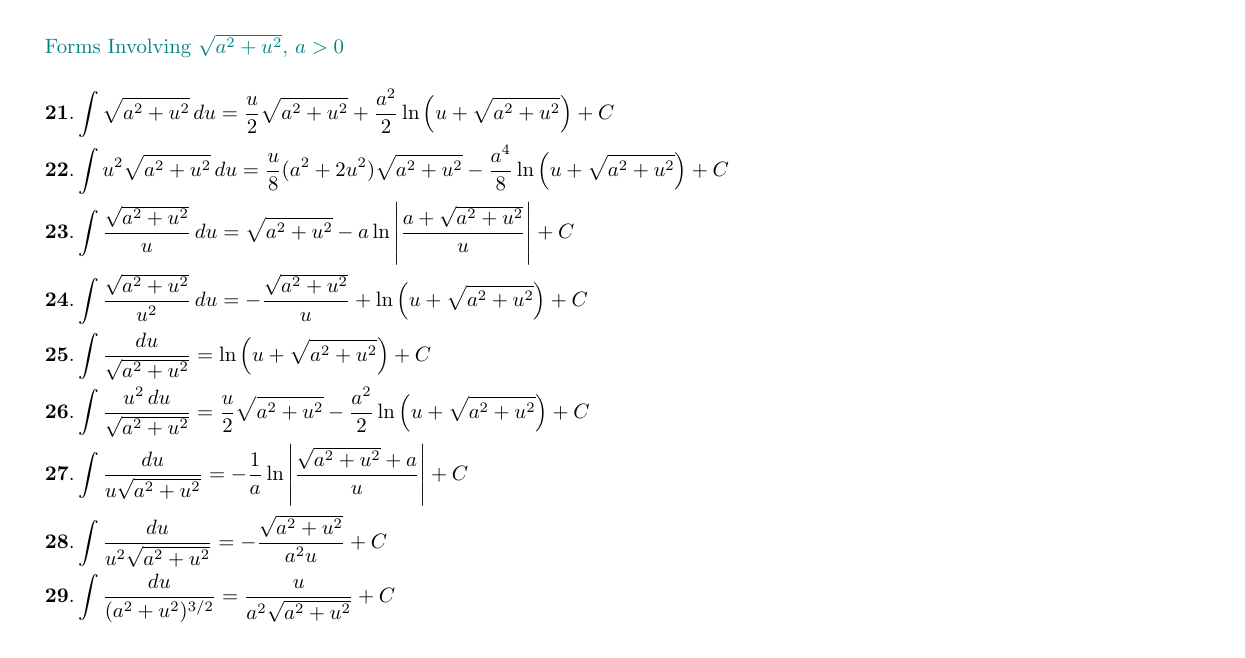
\begin{tikzpicture}[>=latex,xscale=.5*1, yscale=.5*1][font=\sf\normalsize]
\node[scale=0.75] at (0,0) {
$\begin{array}{ll}
\hbox{\color{teal}\rm Forms Involving $\sqrt{a^2+u^2}$, $a > 0$} & \\[3ex]
{\bf 21.}\displaystyle \int \sqrt{a^2+u^2} \, du
= \frac{u}{2} \sqrt{a^2+u^2} + \frac{a^2}{2} \ln \left( u + \sqrt{a^2+u^2}\right) + C
&{\bf}\\[2ex]
{\bf 22.}\displaystyle \int u^2 \sqrt{a^2+u^2} \, du
= \frac{u}{8} (a^2+2u^2) \sqrt{a^2+u^2} - \frac{a^4}{8} \ln \left( u + \sqrt{a^2+u^2}\right) + C \hskip3in{}
&{\bf}\\[2ex]
{\bf 23.}\displaystyle \int \frac{\sqrt{a^2+u^2}}{u} \, du
= \sqrt{a^2+u^2} - a \ln \left| \frac{a + \sqrt{a^2+u^2}}{u}\right| + C
&{\bf}\\[3ex]
{\bf 24.}\displaystyle \int \frac{\sqrt{a^2+u^2}}{u^2} \, du
= -\frac{\sqrt{a^2+u^2}}{u} + \ln \left( u + \sqrt{a^2+u^2}\right) + C
&{\bf}\\[2ex]
{\bf 25.}\displaystyle \int \frac{du}{\sqrt{a^2+u^2}}
= \ln \left( u + \sqrt{a^2+u^2}\right) + C
&{\bf}\\[2ex]
{\bf 26.}\displaystyle \int \frac{u^2 \, du}{\sqrt{a^2+u^2}}
= \frac{u}{2} \sqrt{a^2+u^2} - \frac{a^2}{2} \ln \left( u + \sqrt{a^2+u^2}\right) + C
&{\bf}\\[2ex]
{\bf 27.}\displaystyle \int \frac{du}{u\sqrt{a^2+u^2}}
= - \frac{1}{a} \ln \left| \frac{\sqrt{a^2+u^2}+a}{u}\right| + C
&{\bf}\\[3ex]
{\bf 28.}\displaystyle \int \frac{du}{u^2 \sqrt{a^2+u^2}}
= -\frac{\sqrt{a^2+u^2}}{a^2 u} + C
&{\bf}\\[2ex]
{\bf 29.}\displaystyle \int \frac{du}{(a^2+u^2)^{3/2}}
= \frac{u}{a^2 \sqrt{a^2+u^2}} + C
&{\bf}
\end{array}
$
};

\end{tikzpicture}
\end{document}